\subsection{Temperatuursensor}
De temperatuursensor wordt gebruikt om voor de temperatuurafhankelijkheid van de ISFET te compenseren. Deze sensor bevindt zich aan het begin van de temperatuur signaalverwerking van het systeem, zoals te zien is in \cref{fig:tempInSchema}.

\begin{figure}[!htb]
    \centering
    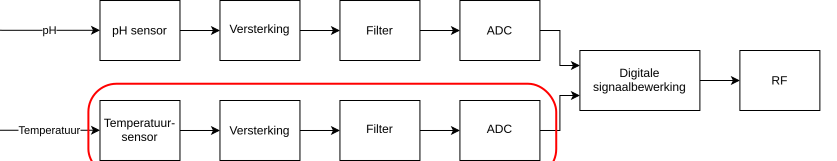
\includegraphics[width=0.95\textwidth]{signaalblokjes/tempInSchema}
    \caption{Het blokschema van de signaalverwerking, met de temperatuursensor omcirkeld.}
    \label{fig:tempInSchema}
\end{figure}

Vanwege tijdsgebrek is dit gedeelte van het systeem echter niet verder ontworpen. De volgende ontwerpfase zal hier verder op in moeten gaan.